\subsection{Individual Filter and Optimizer Ablations}
\label{sec:eval:individual_ablation}

We test the filter checks on the 360 Gemma responses from the matched-context study and the 180 responses from the receipt follow-up. Each response is rescored under eight configurations: all checks, each of five checks removed, duplicate and cardinality checks removed together, and all checks removed. These 4,320 scored outputs share 540 model responses. Candidate order stays fixed. Joint removal tests whether cardinality masks the duplicate check.

Table~\ref{tab:gate_checks} reports full-filter F1 minus each modified-filter F1. We average the paired changes over the three generation arms within each document, then over documents. The filter rejects 28 candidate occurrences, all absent from the references: 11 have the wrong document head and 17 fail source support. Other checks remove no additional candidates. On natural inputs, source support contributes 0.505 F1 points and the head check 0.085 points. Their exploratory effects do not pass Holm correction across the 21 cohort/check comparisons. The response-level audit also records any correct fact displaced when a check is removed.

\begin{table}[t]
\centering
\caption{Paired F1 contribution of filter checks, in percentage points. Each cohort contains 60 documents with three generation arms. Positive values favour the full filter.}
\label{tab:gate_checks}
\small
\begin{tabular}{lrrr}
\toprule
Removed check(s) & Controlled & Natural & Receipts \\
\midrule
Duplicate & +0.000 & +0.000 & +0.000 \\
Document head & +0.037 & +0.085 & +0.000 \\
Relation type & +0.000 & +0.000 & +0.000 \\
Source support & +0.037 & +0.505 & +0.060 \\
Cardinality & +0.000 & +0.000 & +0.000 \\
Duplicate + cardinality & +0.000 & +0.000 & +0.000 \\
All checks & +0.073 & +0.590 & +0.060 \\
\bottomrule
\end{tabular}
\end{table}

\paragraph{Sequential optimizer components.}
The frozen version-1 study replays 13 settings on the same fixed proposals for 225 controlled and 225 natural graphs, giving 5,850 outcomes. Every setting starts from the same preprocessed graph. The reference uses an always-on uniform prior. The learned-prior arm keeps its trigger on; the next arm restores the learned trigger. The remaining arms each change one component of the uniform reference. Table~\ref{tab:optimizer_complete} gives scores and accepted action counts.

\begin{table}[t]
\centering
\caption{Executed optimizer ablations with fixed proposals. Accepted counts are edit bundles/actions, shown as controlled / natural.}
\label{tab:optimizer_complete}
\small
\begin{tabular}{lrrr}
\toprule
Setting & Controlled F1 & Natural F1 & Accepted \\
\midrule
Always-on uniform & 0.8472 & 0.8833 & 0 / 9 \\
Learned prior, always on & 0.8472 & 0.8833 & 0 / 9 \\
Learned prior and trigger & 0.8472 & 0.8833 & 0 / 9 \\
No prior penalty & 0.8472 & 0.8833 & 0 / 9 \\
No action cost & 0.8930 & 0.8813 & 68 / 12 \\
No density bound & 0.8472 & 0.8833 & 0 / 9 \\
No quality bounds & 0.8472 & 0.8833 & 0 / 9 \\
One iteration & 0.8472 & 0.8833 & 0 / 9 \\
No rule candidates & 0.8472 & 0.8833 & 0 / 9 \\
Rule candidates only & 0.8472 & 0.8799 & 0 / 0 \\
No local score/bounds & 0.8472 & 0.8799 & 0 / 0 \\
No graph score/bound & 0.8472 & 0.8833 & 0 / 9 \\
No source score/bound & 0.8472 & 0.8799 & 0 / 9 \\
\bottomrule
\end{tabular}
\end{table}

The local, graph, and source score ablations zero the named quality terms and remove their bounds. Remaining weights keep their original values. Violation detectors, hard-violation reward, candidate generation, and stopping rules remain active. These settings isolate score and bound components. The no-quality-bounds arm removes lower-bound and regression checks while retaining density and empty-graph protection.

On controlled inputs, removing action cost raises F1 from 84.72\% to 89.30\% and defect repair from 32.00\% to 46.89\%. It accepts 68 edits; the reference accepts none. Among the reference\textquotesingle s 220 candidate trials, 218 have non-positive utility and two fail source-quality checks. In another 86 documents, the optimizer stops because it detects no violation. Thus both the stopping profile and the action score limit field restoration.

On natural inputs, removing cost changes F1 from 88.33\% to 88.13\%, with 12 accepted edits instead of nine. More edits therefore do not consistently improve reference accuracy. Removing local or source score/bounds reduces F1 to 87.99\%. The learned prior, learned trigger, density bound, quality bounds, and one-step horizon leave output scores unchanged in this replay. The saved neural weights have the training-feature mismatch discussed in the execution audit; these frozen comparisons measure their runtime effect.
The version-2 study below uses a retrained shared-feature model. Per-candidate traces retain trial graphs, quality profiles, utilities, constraint decisions, and stop reasons.

\begin{figure}[t]
\centering
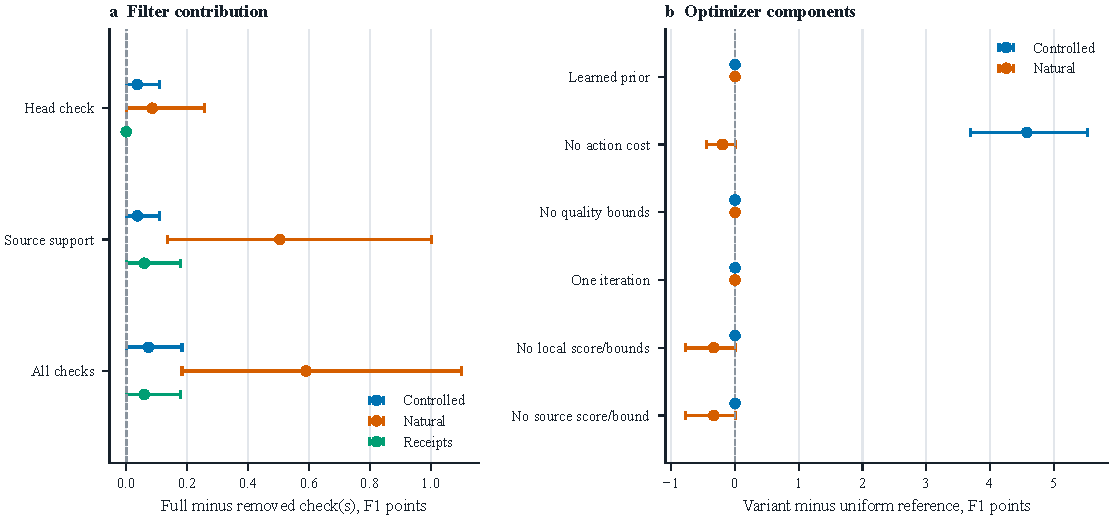
\includegraphics[width=0.98\textwidth]{figure/experiments/individual_ablation.pdf}
\caption{Completed offline ablations. Left: paired F1 contribution of head, source-support, and all filter checks, averaged within each document across generation arms. Right: F1 changes from the always-on uniform optimizer for selected component removals. Bars are marginal 95\% document-bootstrap intervals. All 13 optimizer configurations are reported in Table~\ref{tab:optimizer_complete}.}
\label{fig:individual_ablation}
\end{figure}

\paragraph{Shared-feature retraining and revised execution.}
The version-2 router retains the $8\!\rightarrow\!32\!\rightarrow\!16$
network with one repair head and three scope outputs (884 parameters),
seed 42, and the original document-group split. Training fits the scaler
only on the 2,098 training rows; validation and test each contain 450 rows.
Repair classification and dominant-scope accuracy are 100\% on this
controlled test split. The repair Brier score is $1.02\times10^{-9}$.
These labels follow the known corruption construction; the result measures
recognition of those defects.

\begin{table}[t]
\centering
\caption{Version-2 selector on the same archived proposals. Relative priors use the uniform distribution as their zero point. Accepted edits are controlled / natural.}
\label{tab:math_revision_selector}
\small
\begin{tabular}{lrrr}
\toprule
Prior / offset & Controlled F1 & Natural F1 & Accepted \\
\midrule
Uniform / absolute & 0.8472 & 0.8833 & 0 / 10 \\
Uniform / relative & 0.8472 & 0.8833 & 0 / 10 \\
Learned / absolute & 0.8472 & 0.8799 & 0 / 10 \\
Learned / relative & 0.8929 & 0.8764 & 156 / 51 \\
\bottomrule
\end{tabular}
\end{table}


We execute four fixed router/utility combinations on the same 225 controlled
and 225 natural-input proposals (1,800 outcomes). Table~\ref{tab:math_revision_selector}
reports the revised implementation separately from the frozen component study
above. The revised uniform default evaluates 471 controlled candidate trials,
compared with 220 previously, but still accepts no edits. Candidate evaluation
alone therefore does not remove the positive-utility barrier.
With the retrained prior, the relative offset raises controlled F1 from
84.72\% to 89.29\%, while natural-input F1 changes from 87.99\% to 87.64\%.
The uniform alternatives give identical outputs. The default absolute offset
is retained; the contrast shows that a threshold shift can help one cohort
and harm another. The empty-value diagnostic fix changes no archived case.
All these proposals were previously evaluated, so this is a fixed-candidate
execution comparison. It does not alter the main one-call repair results.

\begin{figure}[t]
\centering
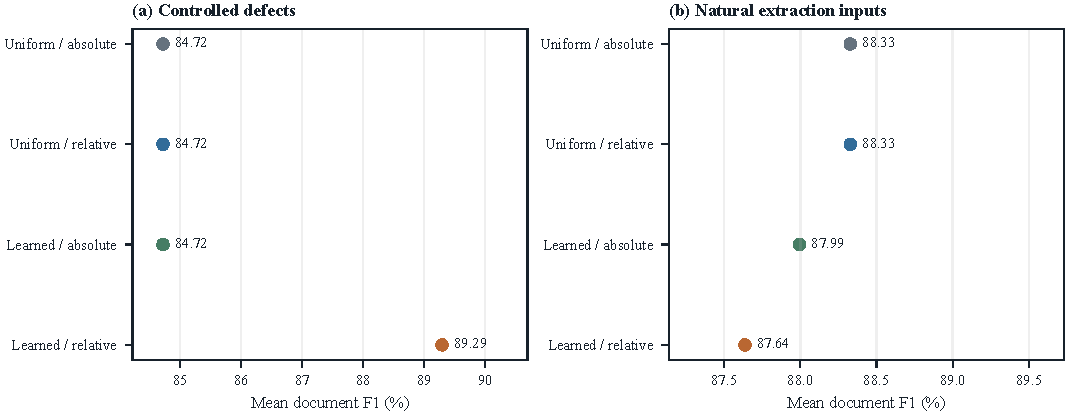
\includegraphics[width=0.98\textwidth]{figure/experiments/math_revision.pdf}
\caption{Revised selector with shared training and execution features. Points
show mean document F1 for fixed prior and offset choices on archived proposals.}
\label{fig:math_revision}
\end{figure}

